%! TeX program = lualatex
\documentclass[12pt]{article}

\usepackage{cmap}
\usepackage{minted}
\usepackage{caption}

\setminted{
    linenos,                % показывать номера строк
    breaklines,             % переносить длинные строки
    breakanywhere=true,     % переносить в любом месте
    tabsize=2,              % размер табуляции
    fontsize=\scriptsize,        % размер шрифта
    frame=lines,            % рамка сверху и снизу
    framesep=2mm,           % расстояние текста от рамки
    baselinestretch=1.1,    % межстрочный интервал
    autogobble=true,        % автоудаление общего отступа
    % xleftmargin=10pt,       % отступ слева
    % numbersep=5pt,          % расстояние между номерами и кодом
}

\usepackage[english, russian]{babel}

\usepackage[nopatch=footnote]{microtype}

\usepackage{float}
\usepackage{fontspec}
\usepackage[pdfborder={0 0 0}]{hyperref}

\usepackage{enumitem}

\setmainfont{TimesNewerRoman}[
  Extension = .otf,
  Path = /nix/store/ihdqrn4p54awd89vrday9k53s8i47bbv-times-newer-roman-unstable-2018-09-11/share/fonts/opentype/,
  UprightFont = *-Regular,
  BoldFont = *-Bold
]
\setmonofont{Ubuntu Mono}

\newcommand{\icon}[1]{\fontspec{UbuntuNerdFont}[Extension = .ttf,
  Path = /nix/store/h721jafy2n74x4k5p0hxbz722h0rncmx-nerd-fonts-ubuntu-3.3.0+0.83/share/fonts/truetype/NerdFonts/Ubuntu/,
  UprightFont = *-Regular,
BoldFont = *-Bold] #1}

\newcommand{\iicon}[1]{{\icon{#1}}}

\usepackage{graphicx}
\usepackage{fontawesome5} % Для иконок

\usepackage[left=2.0cm, right=2.0cm, top=1.0cm, bottom=1.0cm, includeheadfoot]{geometry}

% \usepackage[mocha, textcolor=true, pagecolor=true]{catppuccinpalette} \usemintedstyle{catppuccin-mocha}
\usepackage[latte, textcolor=true, pagecolor=true]{catppuccinpalette} \usemintedstyle{catppuccin-latte}

\usepackage{setspace}
\onehalfspacing

\usepackage{fancyhdr}
\fancyhf{}

\renewcommand{\sectionmark}[1]{\markboth{#1}{}}
\renewcommand{\subsectionmark}[1]{\markright{#1}}

% Настройка колонтитулов
\fancyhead[RO]{\rightmark}
\fancyhead[LO]{\leftmark}

\fancyfoot[L]{\hspace{8pt} \rule{\textwidth}{0.4pt}}
\fancyfoot[R]{\LARGE{\thepage}}
\fancyfoot[C]{}

\newcommand{\lablogo}
{
\begin{center}
    \huge{\textbf{Лабораторная работа №3}} \\
\end{center}
}

\newcommand{\colorURL}[1]{\textcolor{CtpBlue}{#1}}
\newcommand{\colorGIT}[1]{\textcolor{CtpLavender}{#1}}
\renewcommand{\texttt}[1]{{\small\ttfamily #1}}

\setlength{\headheight}{15.2pt}

\DeclareCaptionLabelFormat{gostfigure}{Рисунок #2}
\captionsetup[figure]{labelformat=gostfigure, labelsep=endash}

\DeclareCaptionLabelFormat{gostlisting}{Листинг #2}
\captionsetup[listing]{labelformat=gostlisting, labelsep=endash}

\usepackage{amsmath}
\numberwithin{listing}{section}
\numberwithin{figure}{section}

\usepackage{tocloft}
\renewcommand{\cftsecleader}{\cftdotfill{\cftdotsep}}

\begin{document}

\pagestyle{empty}

\lablogo

\tableofcontents
\newpage
\renewcommand\listoflistingscaption{Листинг}
\listoflistings

\newpage

\pagestyle{fancy}

\newpage

\lablogo

\begin{center}
	\section{ЗАДАНИЕ \ \texorpdfstring{\faScroll}{}}
\end{center}

% \begin{center}
% \begin{minipage}{0.85\linewidth}
\noindent Система управления заказами для онлайн-магазина:
\begin{enumerate}
	\item Реализовать \texttt{WPF} приложение.
	\item Реализовать визуальное отображение списка товаров и списка заказов.
	\item Реализовать функционал добавления, редактирования, удаления конкретных товаров, а также учёт их количества. Реализовать функции уменьшения количества товаров при добавлении их в заказ.
	\item Реализовать функционал добавления, редактирования, удаления заказов, а также возможность редактирования количества товаров, добавленных в заказ.
	\item В списке заказов отобразить информацию о названии, дате (времени) заказа, общей сумме заказа и список входящих в него товаров и их количества.
	\item Реализовать функцию расчёта остатков товара (при уменьшении количества товара в заказе, должно увеличиваться количество товара на складе (возвращаться). При удалении товара из заказа также количество остатков должно увеличиваться (если было куплено 6 единиц товара и заказ удален (отменен), на складе должно стать на 6 единиц товара больше (вернуться))).
\end{enumerate}
Весь код доступен в \colorURL{\href{https://github.com/WebMasterIT/Csharp_Labs/tree/main}{репозитории на GitHub}\ \faGithub}\footnote{Ссылки, выделенные \colorURL{голубым} цветом, ведут на внешние ресурсы; ссылки, выделенные \colorGIT{светло-синим} цветом, указывают на исходный код в репозитории GitHub \ \faGithub.}
% \end{minipage}
% \end{center}

\newpage

\lablogo

\begin{center}
	\subsection{ВАРИАНТЫ ЗАДАНИЙ \ \texorpdfstring{\faTasks}{}}
\end{center}

\begin{enumerate}
	\item Музыкальный магазин
	      \begin{itemize}
		      \item Товары: гитары, синтезаторы, барабаны (поля: \texttt{Name}, \texttt{Price}, \texttt{Stock}, \texttt{Id})
		      \item Заказы: имя клиента, дата, список инструментов
		      \item Создать раздел «Инструменты», добавить поле «Тип» (например, струнные, клавишные)
	      \end{itemize}

	\item Книжный магазин
	      \begin{itemize}
		      \item Товары: книги (поля: \texttt{Name} -- название, \texttt{Price}, \texttt{Stock}, \texttt{Id})
		      \item Заказы: имя клиента, дата, список книг
		      \item Создать раздел «Книги», добавить поле «Автор» в \texttt{Product}
	      \end{itemize}

	\item Магазин электроники
	      \begin{itemize}
		      \item Товары: смартфоны, ноутбуки, наушники
		      \item Заказы: имя клиента, дата, список гаджетов
		      \item Создать раздел «Гаджеты», добавить поле «Бренд» (например, Apple, Samsung)
	      \end{itemize}


	\item Спортивный магазин
	      \begin{itemize}
		      \item Товары: кроссовки, тренажёры, мячи
		      \item Заказы: имя клиента, дата, список товаров
		      \item Создать раздел «Спортинвентарь», добавить поле «Категория» (обувь, оборудование)
	      \end{itemize}

	\item Магазин одежды
	      \begin{itemize}
		      \item Товары: футболки, джинсы, куртки
		      \item Заказы: имя клиента, дата, список одежды
		      \item Создать раздел «Одежда», добавить поле «Размер» (S, M, L)
	      \end{itemize}

	\item Цветочный магазин
	      \begin{itemize}
		      \item Товары: розы, тюльпаны, орхидеи.
		      \item Заказы: имя клиента, дата, список букетов
		      \item Создать раздел \guillemotleft Цветы\guillemotright , добавить поле \guillemotleft Тип\guillemotright \ (букет, горшок)
	      \end{itemize}

	      \newpage

	\item Магазин игрушек
	      \begin{itemize}
		      \item Товары: конструкторы, куклы, машинки.
		      \item Заказы: имя клиента, дата, список игрушек.
		      \item Создать раздел \guillemotleft Игрушки\guillemotright, добавить поле \guillemotleft Возраст\guillemotright.
	      \end{itemize}

	\item Магазин бытовой техники
	      \begin{itemize}
		      \item Товары: холодильники, пылесосы, микроволновки.
		      \item Заказы: имя клиента, дата, список техники.
		      \item Создать раздел \guillemotleft Техника\guillemotright, добавить поле \guillemotleft Мощность\guillemotright
	      \end{itemize}

	\item Магазин косметики
	      \begin{itemize}
		      \item Товары: помады, кремы, духи
		      \item Заказы: имя клиента, дата, список косметики
		      \item Создать раздел «Косметика», добавить поле «Тип» (уход, макияж)
	      \end{itemize}

	\item Магазин автозапчастей
	      \begin{itemize}
		      \item Товары: фильтры, шины, аккумуляторы
		      \item Заказы: имя клиента, дата, список запчастей
		      \item Создать раздел «Запчасти», добавить поле «Марка» (Toyota, BMW)
	      \end{itemize}

	\item Магазин мебели
	      \begin{itemize}
		      \item Товары: диваны, столы, шкафы
		      \item Заказы: имя клиента, дата, список мебели
		      \item Создать раздел «Мебель», добавить поле «Материал» (дерево, металл)
	      \end{itemize}

	\item Магазин канцелярии
	      \begin{itemize}
		      \item Товары: ручки, тетради, маркеры
		      \item Заказы: имя клиента, дата, список товаров
		      \item Создать раздел «Канцелярия», добавить поле «Тип» (письмо, рисование)
	      \end{itemize}

	\item Магазин ювелирных изделий
	      \begin{itemize}
		      \item Товары: кольца, серьги, браслеты
		      \item Заказы: имя клиента, дата, список украшений
		      \item Создать раздел «Украшения», добавить поле «Материал» (золото, серебро)
	      \end{itemize}

	      \newpage

	\item Магазин зоотоваров
	      \begin{itemize}
		      \item Товары: корма, игрушки, клетки
		      \item Заказы: имя клиента, дата, список товаров
		      \item Создать раздел «Зоотовары», добавить поле «Животное» (кошка, собака)
	      \end{itemize}

	\item Магазин видеоигр
	      \begin{itemize}
		      \item Товары: игры для ПК, консолей
		      \item Заказы: имя клиента, дата, список игр
		      \item Создать раздел «Игры», добавить поле «Платформа» (PC, PS5)
	      \end{itemize}

	\item Магазин садовых товаров
	      \begin{itemize}
		      \item Товары: семена, инструменты, горшки
		      \item Заказы: имя клиента, дата, список товаров
		      \item Создать раздел «Садовые товары», добавить поле «Тип» (растения, инструменты)
	      \end{itemize}

	\item Магазин часов
	      \begin{itemize}
		      \item Товары: наручные часы, настенные часы
		      \item Заказы: имя клиента, дата, список часов
		      \item Создать раздел «Часы», добавить поле «Механизм» (кварцевый, механический)
	      \end{itemize}

	\item Магазин обуви
	      \begin{itemize}
		      \item Товары: кроссовки, ботинки, туфли
		      \item Заказы: имя клиента, дата, список обуви
		      \item Создать раздел «Обувь», добавить поле «Размер» (36, 42)
	      \end{itemize}

	\item Магазин настольных игр
	      \begin{itemize}
		      \item Товары: шахматы, монополия, карточные игры
		      \item Заказы: имя клиента, дата, список игр
		      \item Создать раздел «Игры», добавить поле «Игроков» (2-4, 4-8)
	      \end{itemize}

	\item Магазин сувениров
	      \begin{itemize}
		      \item Товары: магниты, статуэтки, открытки
		      \item Заказы: имя клиента, дата, список сувениров
		      \item Создать раздел «Сувениры», добавить поле «Страна» (Россия, Италия)
	      \end{itemize}

	      \newpage

	\item Магазин парфюмерии
	      \begin{itemize}
		      \item Товары: духи, туалетная вода
		      \item Заказы: имя клиента, дата, список парфюма
		      \item Изменения: переименовать «Товары» в «Парфюм», добавить поле «Объём» (50 мл, 100 мл)
	      \end{itemize}

	\item Магазин строительных материалов
	      \begin{itemize}
		      \item Товары: краска, гвозди, доски
		      \item Заказы: имя клиента, дата, список материалов
		      \item Создать раздел «Материалы», добавить поле «Единица» (литры, кг)
	      \end{itemize}

	\item Магазин для художников
	      \begin{itemize}
		      \item Товары: краски, кисти, холсты
		      \item Заказы: имя клиента, дата, список товаров
		      \item Создать раздел «Арт-товары», добавить поле «Тип» (масло, акварель)
	      \end{itemize}

	\item Магазин чая и кофе
	      \begin{itemize}
		      \item Товары: чай, кофе, сиропы
		      \item Заказы: имя клиента, дата, список товаров
		      \item Создать раздел «Напитки», добавить поле «Вес» (100 г, 500 г)
	      \end{itemize}

	\item Магазин для рыбалки
	      \begin{itemize}
		      \item Товары: удочки, приманки, катушки
		      \item Заказы: имя клиента, дата, список товаров
		      \item Создать раздел «Снаряжение», добавить поле «Тип» (спиннинг, фидер)
	      \end{itemize}

	\item Магазин для кемпинга
	      \begin{itemize}
		      \item Товары: палатки, спальники, горелки
		      \item Заказы: имя клиента, дата, список товаров
		      \item Создать раздел «Снаряжение», добавить поле «Вес» (кг)
	      \end{itemize}

	\item Магазин медицинских товаров
	      \begin{itemize}
		      \item Товары: тонометры, бинты, маски
		      \item Заказы: имя клиента, дата, список товаров
		      \item Создать раздел «Медтовары», добавить поле «Назначение» (диагностика, уход)
	      \end{itemize}

	      \newpage

	\item Магазин фильмов
	      \begin{itemize}
		      \item Товары: DVD, Blu-ray диски
		      \item Заказы: имя клиента, дата, список фильмов
		      \item Создать раздел «Фильмы», добавить поле «Жанр» (драма, комедия)
	      \end{itemize}

	\item Магазин горнолыжного оборудования
	      \begin{itemize}
		      \item Товары: сноуборд, горнолыжные костюмы, шлемы
		      \item Заказы: имя клиента, дата, список оборудования
		      \item Создать раздел «Снаряжение», добавить поле «Вид» (сноуборд, лыжи)
	      \end{itemize}

\end{enumerate}

\subsection
[ДОПОЛНИТЕЛЬНОЕ ЗАДАНИЕ~\texorpdfstring{\faLightbulb}{}]
{ДОПОЛНИТЕЛЬНОЕ ЗАДАНИЕ~\texorpdfstring{\faLightbulb}{}\protect\footnotemark}

\begin{enumerate}
	\item[\faTrash] Реализовать удаление единственного товара в заказе. Если в заказе присутствует только один товар, то при его удалении должен удаляться и сам заказ. Количество данного товара должно возвращаться в остаток.

	\item[\faBroom] Добавить функционал снятия выделения товара (в списке выбранных для добавления в заказ) и снятие выделения с заказа при клике по пустому полю (внутри \texttt{listBox}).

\end{enumerate}

\footnotetext{Дополнительные задания выполняются по желанию и не подлежат проверке на зачёте.}

\newpage

\section{ШАГИ ПО СОЗДАНИЮ ПРИЛОЖЕНИЯ ~\texorpdfstring{\faRoute}{}}

\subsection{ШАГ 1: СОЗДАНИЕ ПРОЕКТА}

Для создания проекта необходимо выбрать:
\begin{enumerate}
	\item Создать проект
	\item Приложение \texttt{WPF} (Майкрософт) (Рисунок \ref{fig:projectcreate})

	      \begin{figure}[H]
		      \centering
		      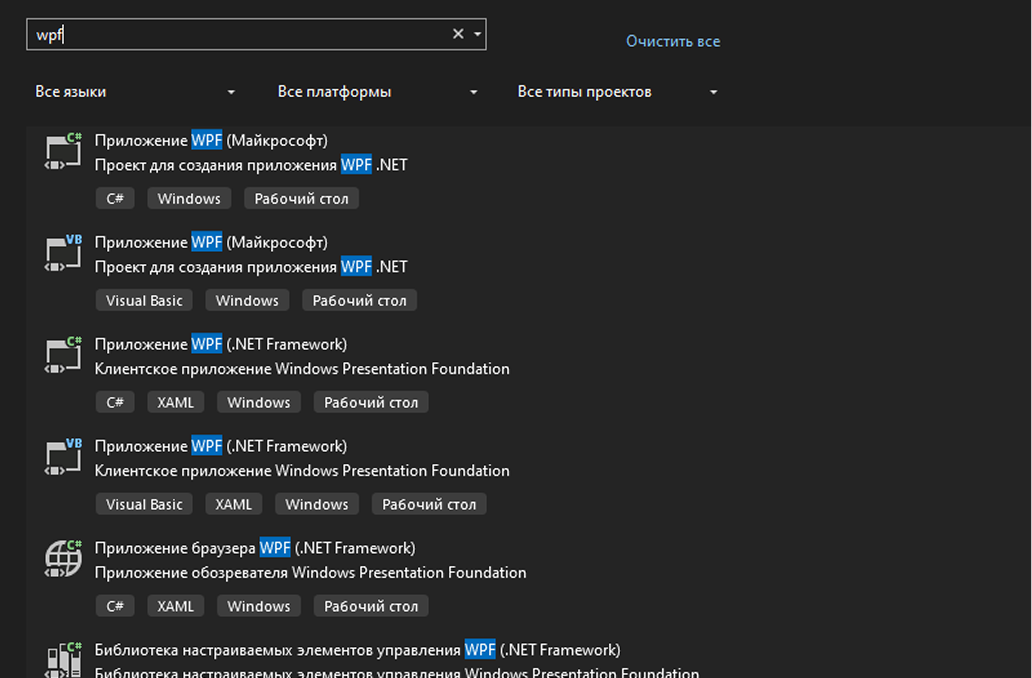
\includegraphics[width=0.55\textwidth]{fig/image 2.png}
		      \caption{Создание проекта}
		      \label{fig:projectcreate}
	      \end{figure}

	\item Далее задать имя проекта: \texttt{StoreManager} (Рисунок \ref{fig:createnameproject})

	      \begin{figure}[H]
		      \centering
		      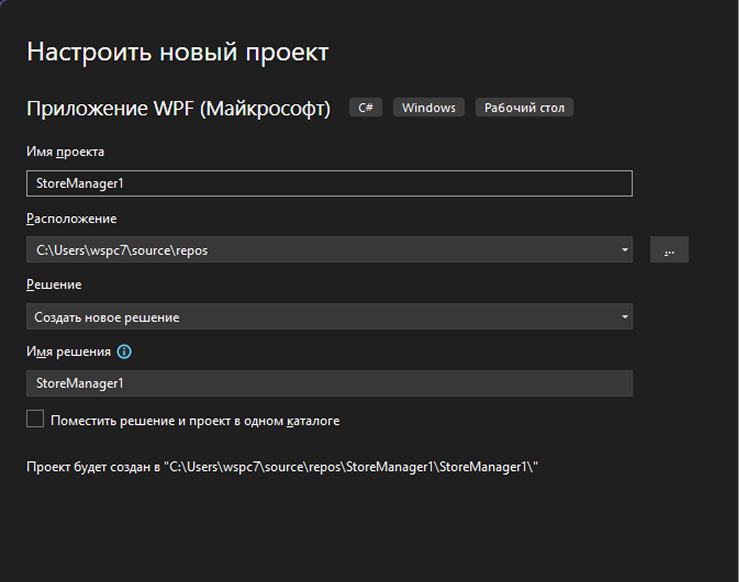
\includegraphics[width=0.55\textwidth]{fig/image 3.png}
		      \caption{Задание имени проекта}
		      \label{fig:createnameproject}
	      \end{figure}

	      \newpage

	\item Выбрать платформу (пример выполнен на .net 8.0) (Рисунок \ref{fig:net8})

	      \begin{figure}[H]
		      \centering
		      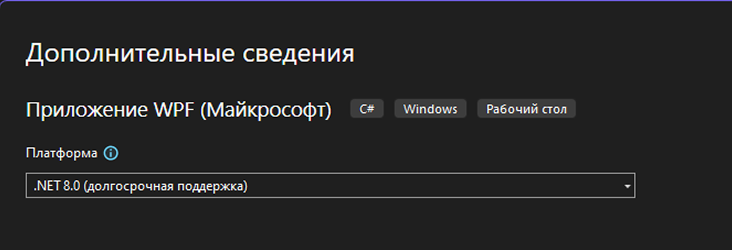
\includegraphics[width=0.8\textwidth]{fig/image 4.png}
		      \caption{Выбор платформы.}
		      \label{fig:net8}
	      \end{figure}

\end{enumerate}

Структура проекта состоит из следующих файлов:

\begin{itemize}
	\item \texttt{App.xaml} -- конфигурация приложения. Определяет основной класс приложения, наследуемый от \texttt{Application}. В нём задаются стили, шаблоны приложения и стартовая точка\footnotemark.
	\item \texttt{App.xaml.cs} -- логика приложения. Содержит класс \texttt{App}, который может переопределять методы, такие как \texttt{OnStartup}, для настройки поведения при запуске, или обрабатывать события приложения.
	\item \texttt{MainWindow.xaml} -- разметка и структура \texttt{UI} (интерфейса) главного окна.
	\item \texttt{MainWindow.xaml.cs} -- логика и обработчики событий окна.
\end{itemize}

\begingroup
\renewcommand{\texttt}[1]{{\scriptsize\ttfamily #1}}
\footnotetext{Обычно указывается начальное окно в свойстве \texttt{StartupUri}}
\endgroup



\newpage

\subsection{ШАГ 2: ДОБАВЛЕНИЕ ФАЙЛОВ}

\begingroup
\renewcommand{\texttt}[1]{{\normalsize\ttfamily #1}}
\stepcounter{subsubsection}
\phantomsection
\addcontentsline{toc}{subsubsection}{\numberline{\thesubsubsection}СОЗДАНИЕ ПАПКИ \texttt{Models}}
\endgroup

Необходимо добавить следующие файлы и папки:
\begin{itemize}
	\item В корне проекта создать папку \texttt{Models}
	\item В папке \texttt{Models} добавить два новых файла классов: \texttt{Product.cs} и \texttt{Order.cs}.
\end{itemize}

\noindent Код для файла \texttt{Order.cs} приведён в листинге \ref{lst:OrderCs}

\begin{listing}[H]
	\inputminted{csharp}{../../3lab/StoreManager/Models/Order.cs}
	\caption{Класс {\colorGIT{\href{https://github.com/WebMasterIT/Csharp_Labs/blob/ec375afd16c0647b337cf3d8a79c8bef904fc1be/3lab/StoreManager/Models/Order.cs\#L1-L27}{Order.cs}}}}
	\label{lst:OrderCs}
\end{listing}

Данный файл отвечает за создание нового объекта заказа. Может содержать уникальные поля, не такие как в примере (в соответствии с вариантом).

\begingroup
\renewcommand{\texttt}[1]{{\normalsize\ttfamily #1}}
\stepcounter{subsubsection}
\phantomsection
\addcontentsline{toc}{subsubsection}{\numberline{\thesubsubsection}КЛАССЫ: \texttt{PRODUCT.CS}, \texttt{ORDER.CS}, \texttt{ORDERITEM.CS}}
\endgroup

Также необходим класс, позволяющий связать товар и его количество в заказе. Пример созданного класса \texttt{OrderItem} и объявления его свойств приведён в листинге \ref{lst:OrderItem}


\begin{listing}[H]
	\inputminted{csharp}{../../3lab/StoreManager/Models/OrderItem.cs}
	\caption{Класс {\colorGIT{\href{https://github.com/WebMasterIT/Csharp_Labs/blob/ec375afd16c0647b337cf3d8a79c8bef904fc1be/3lab/StoreManager/Models/Order.cs\#L1-L27}{Order.cs}}}}
	\label{lst:OrderItem}
\end{listing}

Также необходимо создать файл \texttt{Product.cs}. Данный файл отвечает за создание нового объекта товара. Пример класса \texttt{Product} приведён в листинге \ref{lst:Product.cs}.

\begin{listing}[H]
	\inputminted{csharp}{../../3lab/StoreManager/Models/Product.cs}
	\caption{Класс \colorGIT{\href{https://github.com/WebMasterIT/Csharp_Labs/blob/ec375afd16c0647b337cf3d8a79c8bef904fc1be/3lab/StoreManager/Models/Product.cs\#L1-L18}{Product.cs}}}
	\label{lst:Product.cs}
\end{listing}

\stepcounter{subsubsection}
\phantomsection
\addcontentsline{toc}{subsubsection}{\numberline{\thesubsubsection}ДОБАВЛЕНИЕ КОНВЕРТЕРА}

Также необходимо создать папку \texttt{Converters}. Она будет нужна для создания конвертера. В данной папке нужно создать класс \texttt{BooleanToVisibilityConverter}. Пример кода для данного класса приведён в листинге \ref{lst:BooleanToVisibilityConverter}.

\begin{listing}[H]
	\inputminted{csharp}{../../3lab/StoreManager/Converters/BooleanToVisibilityConverter.cs}
	\caption{Класс \colorGIT{\href{https://github.com/WebMasterIT/Csharp_Labs/blob/ec375afd16c0647b337cf3d8a79c8bef904fc1be/3lab/StoreManager/Converters/BooleanToVisibilityConverter.cs\#L1-L23}{BooleanToVisibilityConverter}}}
	\label{lst:BooleanToVisibilityConverter}
\end{listing}

Этот класс реализует интерфейс \texttt{IValueConverter}, который используется для
преобразования данных при привязке (\texttt{Data Binding})
\begin{itemize}
	\item Метод \texttt{Convert} преобразует значение типа \texttt{bool} в \texttt{Visibility} (перечисление \texttt{WPF} для управления видимостью элементов)
	\item \texttt{true} {\small{{\icon{}}}} \texttt{Visible} (элемент виден)
	\item \texttt{false} {\small{{\icon{}}}} \texttt{Collapsed} (элемент скрыт, не занимает место)
	\item Метод \texttt{ConvertBack} не реализован, так как обратное преобразование не требуется.
\end{itemize}

Конвертеры в \texttt{WPF} используются для преобразования данных между источником
(моделью) и целью (элементом \texttt{UI}). Например, конвертер позволяет адаптировать
значение свойства модели к формату, подходящему для отображения. В данном
случае конвертер применяется для реализации эффекта \texttt{placeholder} (подсказки в
текстовых полях), показывая текст, когда поле пустое (\texttt{Text.IsEmpty}).

Свойство \texttt{Visibility} в \texttt{WPF} имеет три значения:
\begin{itemize}
	\item \texttt{Visible} -- элемент отображается
	\item \texttt{Collapsed} -- элемент скрыт и не занимает места
	\item \texttt{Hidden} -- элемент скрыт, но занимает место в макете.
\end{itemize}

\pagebreak

\subsection{ШАГ 3: РЕАЛИЗАЦИЯ ИНТЕРФЕЙСА}

Для того, чтобы реализовать внешний вид приложения, необходимо добавить
соответствующую разметку в файл \texttt{MainWindow.xaml}.
Пример разметки для данного файла представлен ниже в листинге~\ref{lst:MainWindow}

% \begin{listing}[H]


% TODO: пофиксить листинг
% \captionsetup{type=listing}
\inputminted[firstline=1, lastline=130]{xml}{../../3lab/StoreManager/MainWindow.xaml}
\captionof{listing}{Пример разметки главного окна \colorGIT{\href{https://github.com/WebMasterIT/Csharp_Labs/blob/ec375afd16c0647b337cf3d8a79c8bef904fc1be/3lab/StoreManager/MainWindow.xaml\#L1-L200}{MainWindow}}}
\label{lst:MainWindow}



% \caption{Пример разметки главного окна \colorGIT{\href{https://github.com/WebMasterIT/Csharp_Labs/blob/ec375afd16c0647b337cf3d8a79c8bef904fc1be/3lab/StoreManager/MainWindow.xaml\#L1-L200}{MainWindow}}}
% \end{listing}

\newpage

\subsection{ШАГ 4: РЕАЛИЗАЦИЯ ЛОГИКИ}

Файл \texttt{MainWindow.xaml.cs} -- это \texttt{code-behind} для главного окна приложения. Он содержит логику взаимодействия пользовательского интерфейса (\texttt{UI}) с данными, обрабатывает события (например, нажатия кнопок) и управляет состоянием приложения. Приложение представляет собой систему управления магазином, где пользователь может.

Структура кода состоит из следующих элементов:
\begin{enumerate}
	\item Объявления класса и полей -- определение данных, используемых в приложении.
	\item Конструктора -- инициализация окна и начальных данных.
	\item Методов обновления \texttt{UI} -- синхронизация списков товаров и заказов с \texttt{UI}.
	\item Обработчиков событий -- реакция на действия пользователя (нажатия кнопок, выбор элементов).
	\item Вспомогательных методов -- очистка полей ввода.
\end{enumerate}
В листинге \ref{lst:Main} представлен пример кода для класса \texttt{MainWindow}.

\begin{listing}[H]
	\inputminted[firstline=1, lastline=21]{csharp}{../../3lab/StoreManager/MainWindow.xaml.cs}
	\caption{Пример кода для класса \colorGIT{\href{https://github.com/WebMasterIT/Csharp_Labs/blob/ec375afd16c0647b337cf3d8a79c8bef904fc1be/3lab/StoreManager/MainWindow.xaml.cs\#L1-L21}{MainWindow}}}
	\label{lst:Main}
\end{listing}

Класс \texttt{MainWindow} наследуется от \texttt{Window}, так как это главное окно \texttt{WPF}-приложения. Ключевое слово \texttt{partial} указывает, что класс разделён между \texttt{MainWindow.xaml.cs} (логика) и \texttt{MainWindow\-.xaml} (разметка, сгенерированная часть).

\noindent Поля:
\begin{itemize}
	\item \texttt{products}: Хранит список всех товаров (экземпляры класса \texttt{Product}). Это основная коллекция для управления ассортиментом магазина.
	\item \texttt{orders}: Хранит список заказов (экземпляры класса \texttt{Order}). Каждый заказ содержит имя клиента, дату и список товаров.
	\item \texttt{nextProductId}: Счётчик для генерации уникальных идентификаторов товаров.
\end{itemize}

\noindent Начинается с 1 и увеличивается при добавлении нового товара:
\begin{itemize}
	\item \texttt{nextOrderId}: Аналогичный счётчик для заказов.
	\item \texttt{selectedProductsForOrder}: Временное хранилище товаров (\texttt{OrderItem}), которые пользователь выбрал при формировании нового заказа.
\end{itemize}

Эти поля представляют состояние приложения. Они хранят данные в памяти (вместо базы данных) и используются для отображения в \texttt{UI} и обработки пользовательских действий. Использование \texttt{List<T>} означает, что данные не обновляют \texttt{UI} автоматически (в отличие от \texttt{Observable\-Collection}), поэтому код вручную обновляет списки.

\stepcounter{subsubsection}
\phantomsection
\addcontentsline{toc}{subsubsection}{\numberline{\thesubsubsection}КОНСТРУКТОР}
Далее необходимо объявить основной метод (конструктор) \texttt{MainWindow}.
Пример кода для данного метода представлен в листинге \ref{lst:Main2}

\begin{listing}[H]
	\inputminted[firstline=24, lastline=30]{csharp}{../../3lab/StoreManager/MainWindow.xaml.cs}
	\caption{Пример кода для конструктора класса \colorGIT{\href{https://github.com/WebMasterIT/Csharp_Labs/blob/ec375afd16c0647b337cf3d8a79c8bef904fc1be/3lab/StoreManager/MainWindow.xaml.cs\#L24-L30}{MainWindow}}}
	\label{lst:Main2}
\end{listing}

\texttt{InitializeComponent()} -- метод, автоматически сгенерированный \texttt{WPF}, который загружает разметку из \texttt{MainWindow.xaml}, инициализирует элементы интерфейса (такие как кнопки, списки и текстовые поля) и устанавливает необходимые привязки. Без его вызова пользовательский интерфейс не будет отображён.

\noindent Вызовы методов обновления:
\begin{itemize}
	\item \texttt{UpdateProductList()} -- устанавливает \texttt{ItemsSource} для \texttt{ListBox} с товарами, чтобы отобразить начальный список (пустой на старте).
	\item \texttt{UpdateOrderList()} -- аналогично предыдущему методу, только для списка заказов (\texttt{Or\-dersList}).
	\item \texttt{UpdateSelectedProductsList()} -- обновляет список выбранных товаров для заказа (\texttt{Sel\-ected\-ProductsList}).
\end{itemize}

\noindent Назначение:
\begin{itemize}
	\item Конструктор подготавливает приложение к работе, загружая \texttt{UI} и синхронизируя данные с элементами управления.
	\item Поскольку списки изначально пусты, вызовы обновления предотвращают ошибки отображения.
\end{itemize}

Методы для обновления списков товаров, заказов и выбранных товаров для заказа
представлены в листинге \ref{lst:Method}

\begin{listing}[H]
	\inputminted[firstline=32, lastline=51]{csharp}{../../3lab/StoreManager/MainWindow.xaml.cs}
	\caption{\colorGIT{\href{https://github.com/WebMasterIT/Csharp_Labs/blob/ec375afd16c0647b337cf3d8a79c8bef904fc1be/3lab/StoreManager/MainWindow.xaml.cs\#L32-L51}{Методы}} обновления данных}
	\label{lst:Method}
\end{listing}

Метод \texttt{UpdateProductList} Сбрасывает \texttt{ItemsSource} в \texttt{null}, чтобы очистить привязку. Устанавливает \texttt{ItemsSource} в \texttt{products}, чтобы \texttt{ListBox} (\texttt{ProductsList}) отобразил текущий список товаров. Остальные методы работают аналогично. \texttt{Null} используется для предотвращения проблемы с кэшированием данных в \texttt{WPF}, обеспечивая корректное обновление интерфейса.

\stepcounter{subsubsection}
\phantomsection
\addcontentsline{toc}{subsubsection}{\numberline{\thesubsubsection}РАБОТА С ТОВАРАМИ (ДОБАВЛЕНИЕ, ОБНОВЛЕНИЯ, УДАЛЕНИЕ)}

Далее рассмотрим методы для работы с конкретными товарами. Эти методы реагируют на действия пользователя с товарами (кнопки «Добавить», «Обновить», «Удалить», выбор в списке). Метод добавления нового товара представлен в листинге \ref{lst:MethodAdd}

\begin{listing}[H]
	\inputminted[firstline=53, lastline=80]{csharp}{../../3lab/StoreManager/MainWindow.xaml.cs}
	\caption{\colorGIT{\href{https://github.com/WebMasterIT/Csharp_Labs/blob/ec375afd16c0647b337cf3d8a79c8bef904fc1be/3lab/StoreManager/MainWindow.xaml.cs\#L53-L80}{Метод}} добавления нового товара}
	\label{lst:MethodAdd}
\end{listing}

\noindent Данный метод проверяет валидность ввода:
\begin{itemize}
	\item \texttt{ProductName.Text} не пустое.
	\item Проверяет \texttt{ProductPrice.Text} (что цена корректна (\texttt{decimal})), количество -- неотрицательное число (\texttt{int}).
	\item \texttt{ProductStock.Text} преобразуется в \texttt{int}.
\end{itemize}

Если валидация не пройдена, показывает сообщение об ошибке. Создаёт новый объект \texttt{Product} с уникальным \texttt{Id} (из \texttt{nextProductId}), именем, ценой и запасом из полей ввода. Добавляет товар в список \texttt{products}, обновляет \texttt{UI} (\texttt{Update\-ProductList}) и очищает поля ввода (\texttt{Clear\-ProductFields}).

Следующий метод позволяет обновить (редактировать) информацию о конкретном товаре. Реализация метода обновления представлена в листинге \ref{lst:MethodUpdate}

\begin{listing}[H]
	\inputminted[firstline=82, lastline=110]{csharp}{../../3lab/StoreManager/MainWindow.xaml.cs}
	\caption{\colorGIT{\href{https://github.com/WebMasterIT/Csharp_Labs/blob/ec375afd16c0647b337cf3d8a79c8bef904fc1be/3lab/StoreManager/MainWindow.xaml.cs\#L82-L110}{Метод}} обновления товара}
	\label{lst:MethodUpdate}
\end{listing}

\noindent Данный метод проверяет, выбран ли товар в списке \texttt{ProductsList}.
\begin{itemize}
	\item Проводит валидацию ввода (аналогично методу \texttt{AddProduct\_Click}).
	\item Если товар выбран и данные валидны, обновляет свойства выбранного объекта \texttt{Product} (\texttt{Name}, \texttt{Price}, \texttt{Stock}).
	\item Обновляет \texttt{UI} и очищает поля.
	\item Если товар не выбран, показывает предупреждение.
\end{itemize}

Для того, чтобы исключить конкретный товар из общего списка, используется метод \texttt{Delete\-Product} из листинга \ref{lst:MethodDelete}.


\begin{listing}[H]
	\inputminted[firstline=112, lastline=141]{csharp}{../../3lab/StoreManager/MainWindow.xaml.cs}
	\caption{\colorGIT{\href{https://github.com/WebMasterIT/Csharp_Labs/blob/ec375afd16c0647b337cf3d8a79c8bef904fc1be/3lab/StoreManager/MainWindow.xaml.cs\#L112-L141}{Метод}} удаления товара}
	\label{lst:MethodDelete}
\end{listing}

\noindent Данный метод выполняет следующие функции:
\begin{itemize}
	\item Удаляет товар из списка, если он не используется в заказах.
	\item Если товар выбран и не связан с заказами, запрашивает подтверждение и удаляет его.
	\item Также удаляет его из текущего заказа (если он там есть).
	\item Если товар используется в заказах -- показывает предупреждение.
	\item Обновляет \texttt{UI} и очищает поля.
\end{itemize}


\begin{listing}[H]
	\inputminted[firstline=143, lastline=184]{csharp}{../../3lab/StoreManager/MainWindow.xaml.cs}
	\caption{\colorGIT{\href{https://github.com/WebMasterIT/Csharp_Labs/blob/ec375afd16c0647b337cf3d8a79c8bef904fc1be/3lab/StoreManager/MainWindow.xaml.cs\#L143-L184}{Методы}} редактирования товара и добавления в список выбранных товаров для заказа}
	\label{lst:MethodEdit}
\end{listing}

% NOTE 

Далее рассмотрим методы \texttt{ProductsList\_SelectionChanged} и \texttt{AddToOrder}. Когда пользователь выбирает товар в списке \texttt{ProductsList}, метод \texttt{ProductsList\_SelectionChanged} заполняет поля \texttt{Product\-Name}, \texttt{ProductPrice}, \texttt{ProductStock} данными выбранного товара. Используется также для редактирования информации о товаре (листинг \ref{lst:MethodEdit}).

Метод \texttt{AddToOrder} добавляет выбранный товар из списка в текущий заказ.
Если товар уже добавлен -- увеличивает его количество.
Если нет -- создаёт новую позицию.
Также уменьшает остаток товара на складе.
Обновляет \texttt{UI}.
Если товар не выбран или нет в наличии -- показывает предупреждение.

\stepcounter{subsubsection}
\phantomsection
\addcontentsline{toc}{subsubsection}{\numberline{\thesubsubsection} РАБОТА С ЗАКАЗАМИ (ДОБАВЛЕНИЕ, ОБНОВЛЕНИЕ, УДАЛЕНИЕ)}

Далее рассмотрим метод создания нового заказа. Пример кода для данного метода
представлен в листинге~\ref{lst:MethodAddInList}.

\begin{listing}[H]
	\inputminted[firstline=186, lastline=216]{csharp}{../../3lab/StoreManager/MainWindow.xaml.cs}
	\caption{\colorGIT{\href{https://github.com/WebMasterIT/Csharp_Labs/blob/ec375afd16c0647b337cf3d8a79c8bef904fc1be/3lab/StoreManager/MainWindow.xaml.cs\#L186-L216}{Метод}} добавления заказа}
	\label{lst:MethodAddInList}
\end{listing}

\noindent Данный метод выполняет следующие функции:
\begin{itemize}
	\item Создаёт новый заказ.
	\item Проверяет, введено ли имя клиента и есть ли хотя бы один товар в заказе.
	\item Если всё в порядке -- формирует объект \texttt{Order}, копирует список товаров и добавляет заказ в список \texttt{orders}.
	\item Обновляет \texttt{UI} и очищает поля.
	\item Если что-то не заполнено -- показывает ошибку.
\end{itemize}

Следующий метод позволяет обновить информацию о заказе. Пример кода для данного метода представлен в листинге \ref{lst:MethodUpdate2}.

\begin{listing}[H]
	\inputminted[firstline=218, lastline=266]{csharp}{../../3lab/StoreManager/MainWindow.xaml.cs}
	\caption{\colorGIT{\href{https://github.com/WebMasterIT/Csharp_Labs/blob/ec375afd16c0647b337cf3d8a79c8bef904fc1be/3lab/StoreManager/MainWindow.xaml.cs\#L218-L266}{Метод}} обновления заказа}
	\label{lst:MethodUpdate2}
\end{listing}

\begin{itemize}
	\item Обновляет выбранный заказ.
	\item Проверяет имя клиента и наличие товаров в заказе.
	\item Если данные валидны -- проверяет, есть ли достаточный остаток на складе для всех добавляемых/увеличиваемых товаров.
	\item Если проверки пройдены, обновляет имя клиента, дату и товары в заказе, корректируя запасы на складе (возвращая старые и забирая новые).
	\item Обновляет \texttt{UI} и очищает поля.
	\item Если что-то не так -- показывает сообщение об ошибке.
\end{itemize}

Следующий метод позволяет удалить выбранный заказ. Пример кода для данного метода представлен в листинге \ref{lst:MethodDelete2}.

\begin{listing}[H]
	\inputminted[firstline=268, lastline=295]{csharp}{../../3lab/StoreManager/MainWindow.xaml.cs}
	\caption{\colorGIT{\href{https://github.com/WebMasterIT/Csharp_Labs/blob/ec375afd16c0647b337cf3d8a79c8bef904fc1be/3lab/StoreManager/MainWindow.xaml.cs\#L268-L295}{Метод}} удаления заказа}
	\label{lst:MethodDelete2}
\end{listing}

Данный метод позволяет удалить выбранный заказ и вернуть товары на склад при подтверждении действия пользователем.
Параметры:
\begin{itemize}
	\item \texttt{object sender} — источник события (обычно кнопка).
	\item \texttt{RoutedEventArgs} — аргументы события нажатия.
\end{itemize}
Основная логика:
\begin{enumerate}
	\item Проверка выбора заказа:
	      \begin{itemize}
		      \item Метод сначала проверяет, выбран ли заказ в списке \texttt{OrdersList}.
	      \end{itemize}
	\item Подтверждение действия:
	      \begin{itemize}
		      \item Пользователю выводится диалоговое окно с вопросом, действительно ли он хочет удалить заказ клиента.
		      \item Если пользователь нажимает "Да"\ (\texttt{MessageBoxResult.Yes}), продолжается выполнение.
	      \end{itemize}
	\item Возврат товаров на склад:
	      \begin{itemize}
		      \item Проходит по каждому элементу заказа (\texttt{selectedOrder.Items}) и возвращает соответствующее количество товара на склад (увеличивает \texttt{item.Product.Stock} на \texttt{item.Quantity}).
	      \end{itemize}
	\item Удаление заказа:
	      \begin{itemize}
		      \item Удаляет заказ из списка заказов (\texttt{orders.Remove(selectedOrder)}).
		      \item Обновляет список товаров и заказов, а также очищает поля заказа:
		            \begin{itemize}
			            \item \texttt{UpdateProductList()}
			            \item \texttt{UpdateOrderList()}
			            \item \texttt{ClearOrderFields()}
		            \end{itemize}
	      \end{itemize}
	\item Обработка случая, если заказ не выбран:
	      \begin{itemize}
		      \item Выводит предупреждающее сообщение, прося пользователя выбрать заказ перед удалением.
	      \end{itemize}

\end{enumerate}


Следующий метод нужен для удаления товара из заказа. Код для данного метода представлен в листинге \ref{lst:MethodDelete3}.

\begin{listing}[H]
	\inputminted[firstline=297, lastline=338]{csharp}{../../3lab/StoreManager/MainWindow.xaml.cs}
	\caption{\colorGIT{\href{https://github.com/WebMasterIT/Csharp_Labs/blob/ec375afd16c0647b337cf3d8a79c8bef904fc1be/3lab/StoreManager/MainWindow.xaml.cs\#L297-L338}{Метод}} удаления товара из заказа}
	\label{lst:MethodDelete3}
\end{listing}

\begin{itemize}
	\item Метод \texttt{RemoveProductFromOrder} удаляет товар из текущего заказа (\texttt{selected\-Products\-For\-Order}).
	\item Если количество выбранного \texttt{OrderItem} больше 1 -- уменьшает его.
	\item Если товар выбран -- полностью удаляет позицию (\texttt{OrderItem}) из списка \texttt{selected\-Produc\-ts\-ForOrder}.
	\item Возвращает количество товара на склад.
	\item Если это был единственный товар в редактируемом заказе (\texttt{OrdersList.SelectedItem}), запрашивает подтверждение и удаляет сам заказ.
	\item Обновляет \texttt{UI}.
	\item Если товар не выбран -- показывает предупреждение.
\end{itemize}

\stepcounter{subsubsection}
\phantomsection
\addcontentsline{toc}{subsubsection}{\numberline{\thesubsubsection}ИЗМЕНЕНИЕ КОЛИЧЕСТВА ТОВАРОВ (КНОПКИ \texttt{<<+>>} И \texttt{<<->>})}

Далее рассмотрим методы, отвечающие за увеличение и уменьшение количества
товара в заказе (кнопки \guillemotleft\texttt{+}\guillemotright \ и \guillemotleft\texttt{-}\guillemotright). Пример этих методов представлен в листинге \ref{lst:MethodControl}.

\begin{listing}[H]
	\inputminted[firstline=342, lastline=377]{csharp}{../../3lab/StoreManager/MainWindow.xaml.cs}
	\caption{\colorGIT{\href{https://github.com/WebMasterIT/Csharp_Labs/blob/ec375afd16c0647b337cf3d8a79c8bef904fc1be/3lab/StoreManager/MainWindow.xaml.cs\#L342-L377}{Методы}} управления количеством товара в заказе}
	\label{lst:MethodControl}
\end{listing}

Данный метод позволяет выделить определенный заказ и изменить имя заказчика. Реализация метода представлена на рисунке~\ref{lst:MethodUpdate3}.

\begin{listing}[H]
	\inputminted[firstline=379, lastline=390]{csharp}{../../3lab/StoreManager/MainWindow.xaml.cs}
	\caption{\colorGIT{\href{https://github.com/WebMasterIT/Csharp_Labs/blob/ec375afd16c0647b337cf3d8a79c8bef904fc1be/3lab/StoreManager/MainWindow.xaml.cs\#L379-L390}{Метод}} обновления нового товара }
	\label{lst:MethodUpdate3}
\end{listing}

\begin{itemize}
	\item Срабатывает при выборе заказа из списка.
	\item Заполняет поле имени клиента.
	\item Загружает список товаров из заказа в текущий список \texttt{selectedProductsForOrder}.
	\item Обновляет \texttt{UI}.
\end{itemize}

\stepcounter{subsubsection}
\phantomsection
\addcontentsline{toc}{subsubsection}{\numberline{\thesubsubsection}СБРОС ВЫДЕЛЕНИЯ В СПИСКАХ}

% NOTE

Далее рассмотрим методы очищения полей \texttt{ClearProductFields} и \texttt{ClearOrderFields}. Листинг этих методов приведён в листинге \ref{lst:MethodClear}.

\begin{listing}[H]
	\inputminted[firstline=392, lastline=432]{csharp}{../../3lab/StoreManager/MainWindow.xaml.cs}
	\caption{\colorGIT{\href{https://github.com/WebMasterIT/Csharp_Labs/blob/ec375afd16c0647b337cf3d8a79c8bef904fc1be/3lab/StoreManager/MainWindow.xaml.cs\#L379-L432}{Методы}} очистки полей и сброса выделения товара}
	\label{lst:MethodClear}
\end{listing}

Метод \texttt{ClearProductFields} позволяют очистить текстовые поля для добавления и редактирования товара и снимают выделение в списке товаров. Метод \texttt{ClearOrderFields} очищает поле имени клиента и список выбранных товаров, снимает выделение в списке заказов, при этом не трогает список товаров (оставляет выделение). Метод \texttt{ProductsList\_MouseLeftButtonDown} используется, если пользователь кликнул мышью по пустому месту в списке товаров. В этом случае метод сбрасывает выделение. Применяется для удобства работы — чтобы можно было "отменить"\ выбор.

\pagebreak

\section{ДЕМОНСТРАЦИЯ РАБОТЫ \ \texorpdfstring{\faGlasses}{}}

\subsection{ДОБАВЛЕНИЕ ТОВАРОВ}

В итоговом варианте внешний вид приложения представлен на Рисунке \ref{fig:demo1}

\begin{figure}[ht]
	\centering
	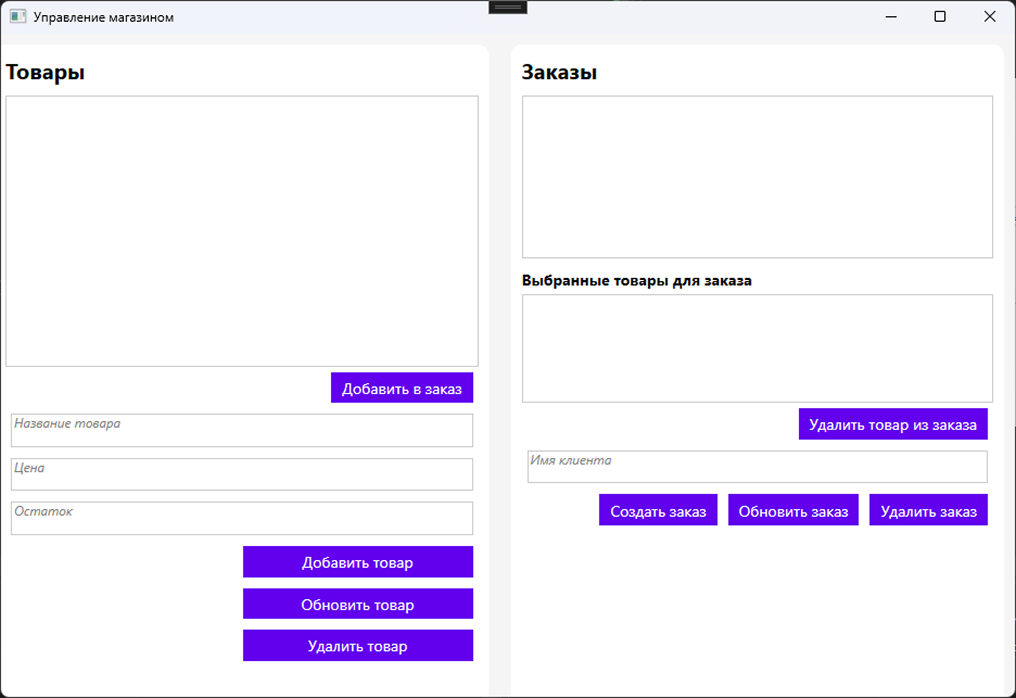
\includegraphics[width=1.0\textwidth]{fig/image 26.png}
	\caption{Интерфейс приложения}
	\label{fig:demo1}
\end{figure}

\pagebreak


\subsection{ДОБАВЛЕНИЕ ТОВАРОВ В ЗАКАЗ}

В качестве примера отображения информации в приложении, введены данные о товарах и заказе. Пример интерфейса приложения с введенными данными приведен на Рисунке \ref{fig:demo2}

\begin{figure}[ht]
	\centering
	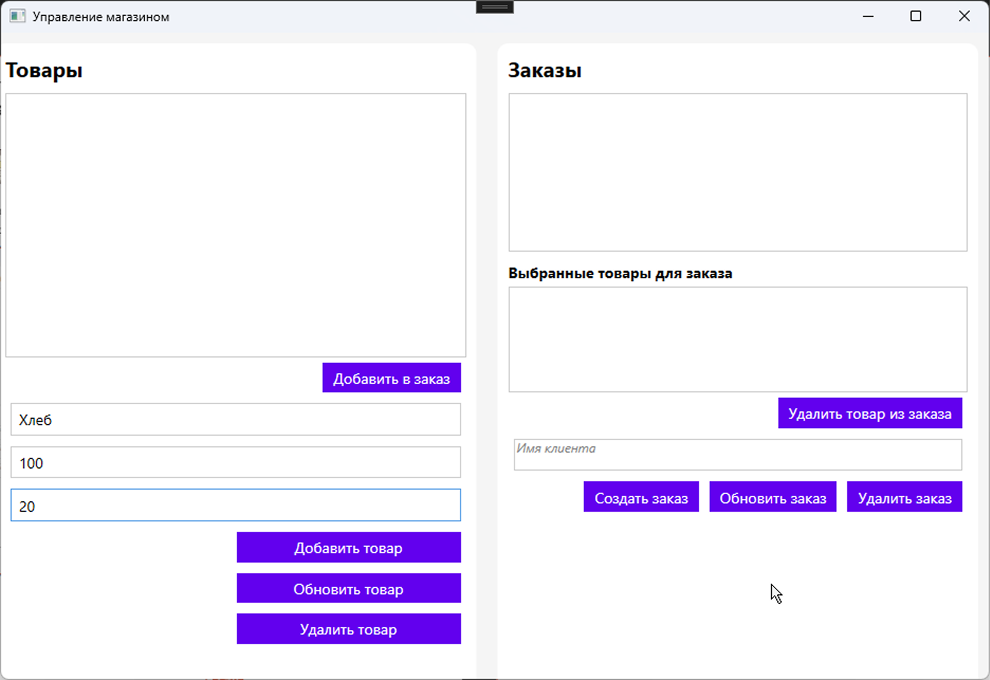
\includegraphics[width=1.0\textwidth]{fig/image 27.png}
	\caption{Пример заполнения информации в приложении}
	\label{fig:demo2}
\end{figure}

\pagebreak

\subsection{СОЗДАНИЕ ЗАКАЗА}

Далее по нажатию кнопки "Добавить товар", товар добавляется в общий список. Таким образом можно добавить группу товаров (Рисунок \ref{fig:demo3}).

\begin{figure}[ht]
	\centering
	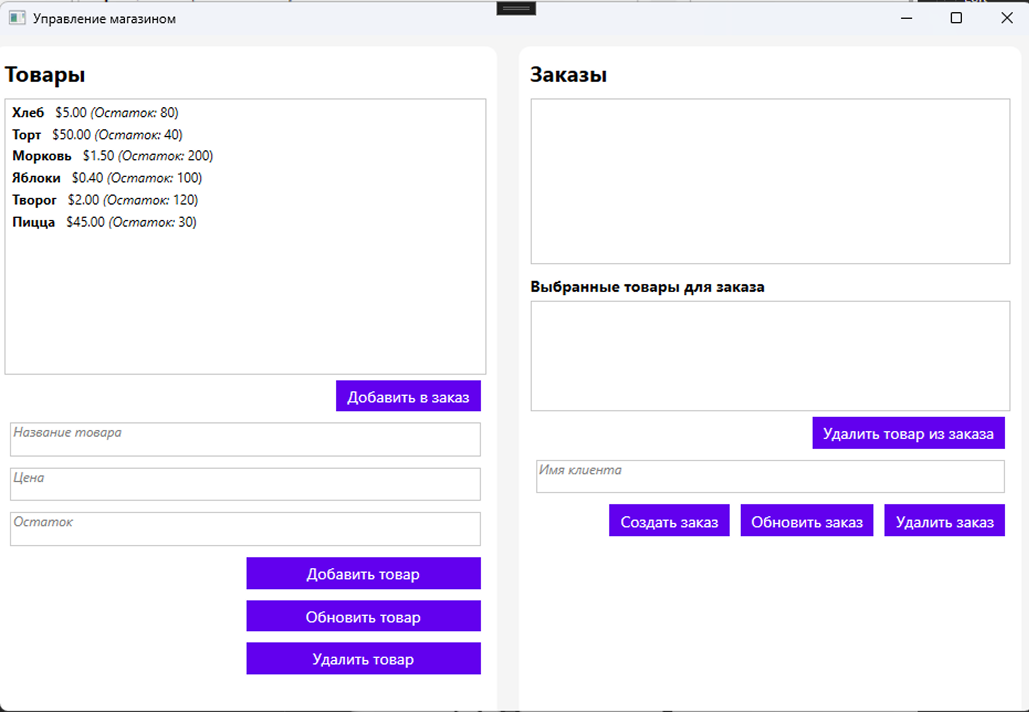
\includegraphics[width=1.0\textwidth]{fig/image 60.png}
	\caption{Пример добавления группы товаров}
	\label{fig:demo3}
\end{figure}

\pagebreak

\subsection{ПРОСМОТР СОДЕРЖИМОГО ЗАКАЗА}

Далее необходимо выбрать конкретный товар из списка, по нажатию кнопки добавить его в список выбранных товаров. В данном списке с помощью кнопки \guillemotleft\texttt{+}\guillemotright \ и \guillemotleft\texttt{-}\guillemotright \ можно отредактировать количество товаров для добавления в заказ (Рисунок \ref{fig:demo4}).


\begin{figure}[ht]
	\centering
	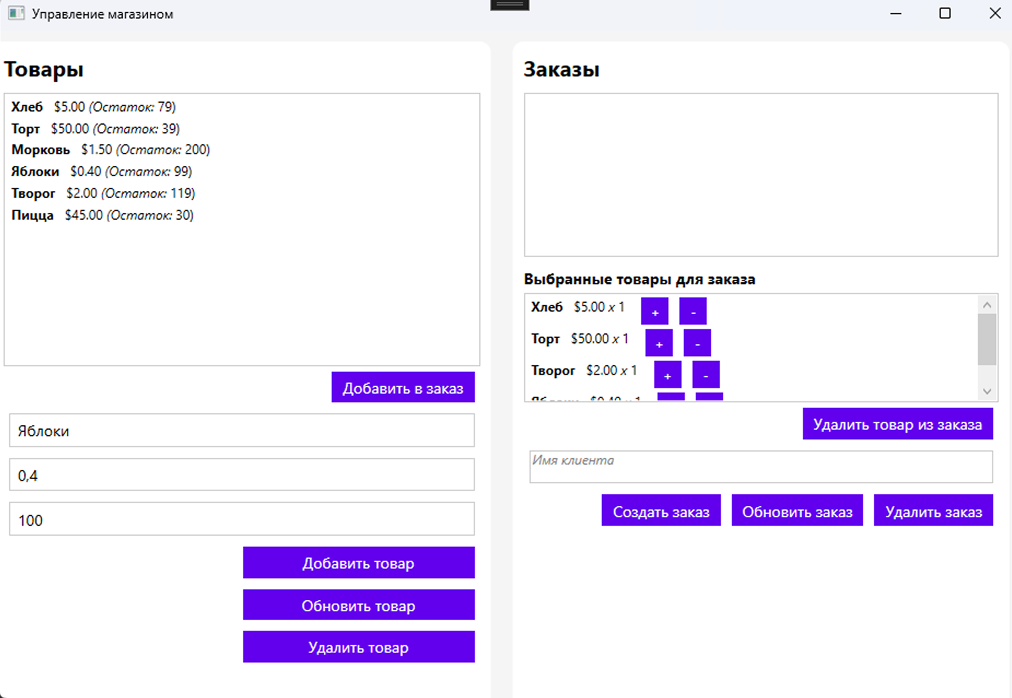
\includegraphics[width=1.0\textwidth]{fig/image 61.png}
	\caption{Пример добавления товаров в заказ} % Updated caption
	\label{fig:demo4}
\end{figure}

\pagebreak

\subsection{УДАЛЕНИЕ ТОВАРОВ ИЗ ЗАКАЗА}

Далее необходимо ввести имя клиента (название заказа) и нажать кнопку \guillemotleft Создать заказ\guillemotright \ для добавления нового заказа в список заказов (Рисунок \ref{fig:demo5}).


\begin{figure}[ht]
	\centering
	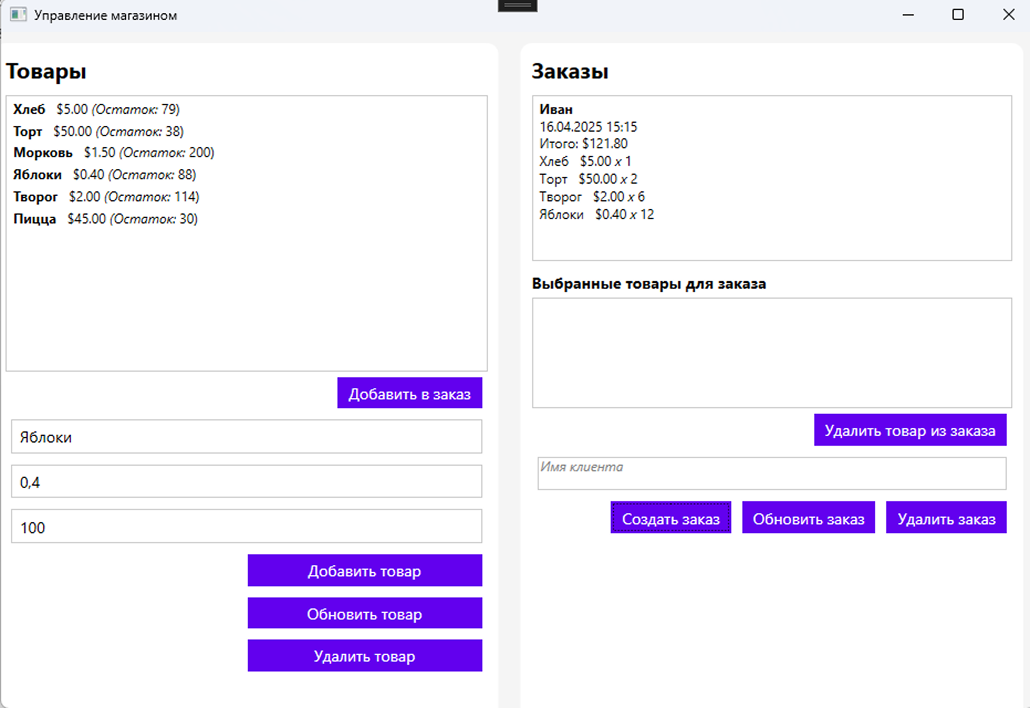
\includegraphics[width=1.0\textwidth]{fig/image 62.png}
	\caption{Пример создания заказа} % Updated caption
	\label{fig:demo5}
\end{figure}

\pagebreak

\subsection{ОБНОВЛЕНИЕ И УДАЛЕНИЕ ЗАКАЗОВ}

При нажатии на конкретный заказ можно вывести список товаров (Рисунок \ref{fig:demo6}).

\begin{figure}[ht]
	\centering
	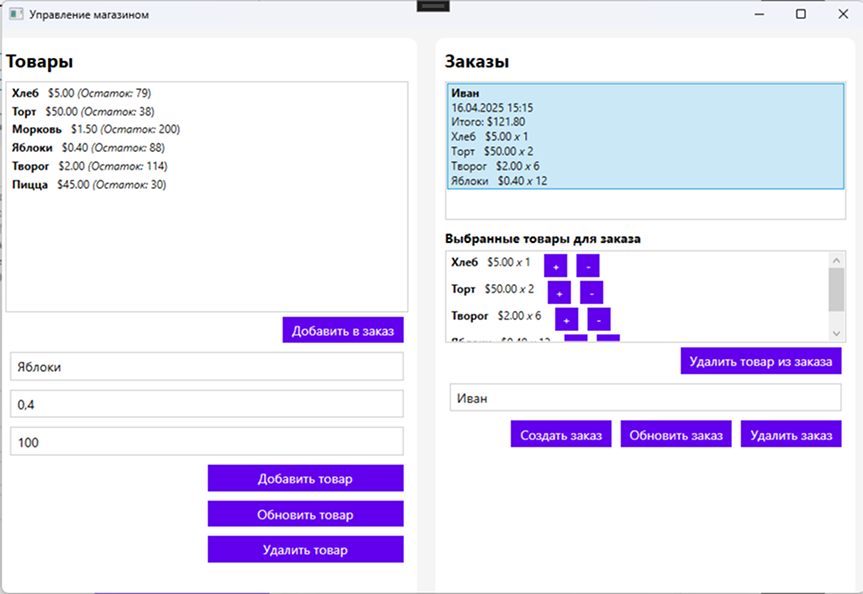
\includegraphics[width=1.0\textwidth]{fig/image 63.png}
	\caption{Вывод списка товаров в заказе}
	\label{fig:demo6}
\end{figure}

\pagebreak


При нажатии кнопки «Удалить товар из заказа» можно удалить конкретный товар, добавленный в заказ (Рисунок \ref{fig:demo7}).

\begin{figure}[ht]
	\centering
	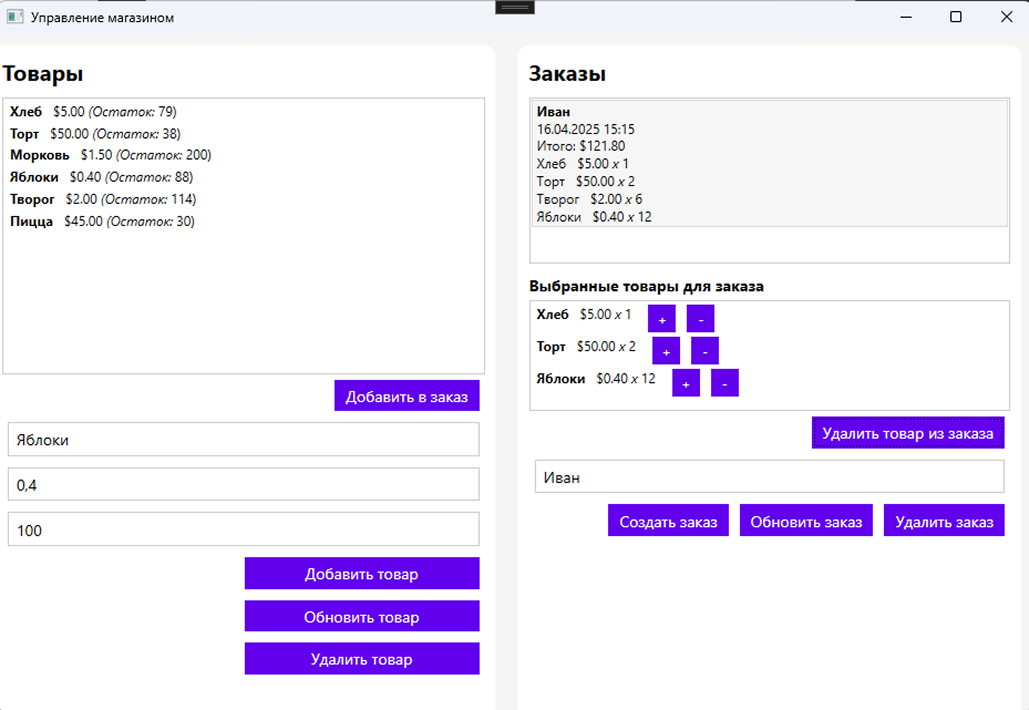
\includegraphics[width=1.0\textwidth]{fig/image 64.png}
	\caption{Удаление товара из заказа}
	\label{fig:demo7}
\end{figure}

\pagebreak

Кнопка «Обновить заказ» позволяет обновить информацию о заказе и удалить конкретный товар, добавленный в заказ (Рисунок \ref{fig:demo8}).

\begin{figure}[ht]
	\centering
	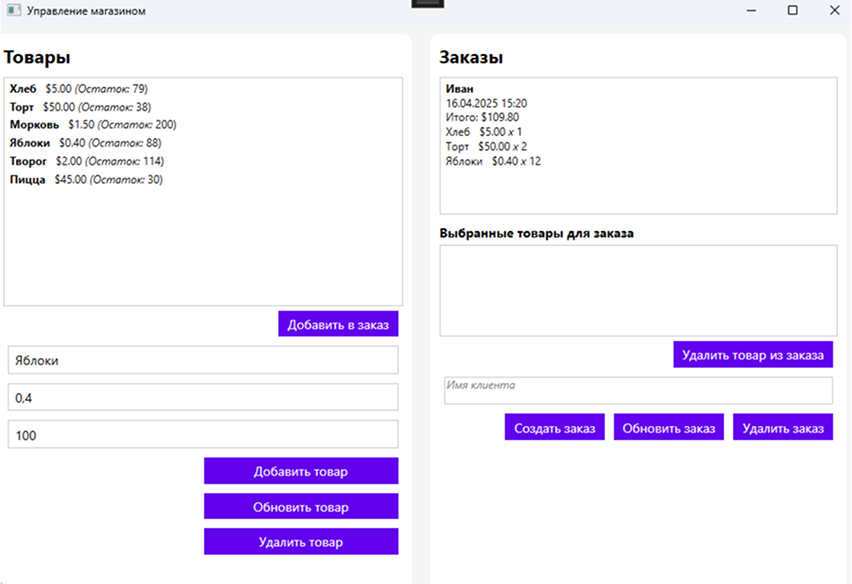
\includegraphics[width=1.0\textwidth]{fig/image 65.png}
	\caption{Обновление списка товаров в заказе}
	\label{fig:demo8}
\end{figure}

\pagebreak

При нажатии кнопки «Удалить заказ» можно удалить конкретный заказ из списка (Рисунок \ref{fig:demo9}). При удалении на экран выводится сообщение с подтверждением. После удаления количество остатков товара увеличивается в соответствии с тем, сколько товара было в заказе.

\begin{figure}[ht]
	\centering
	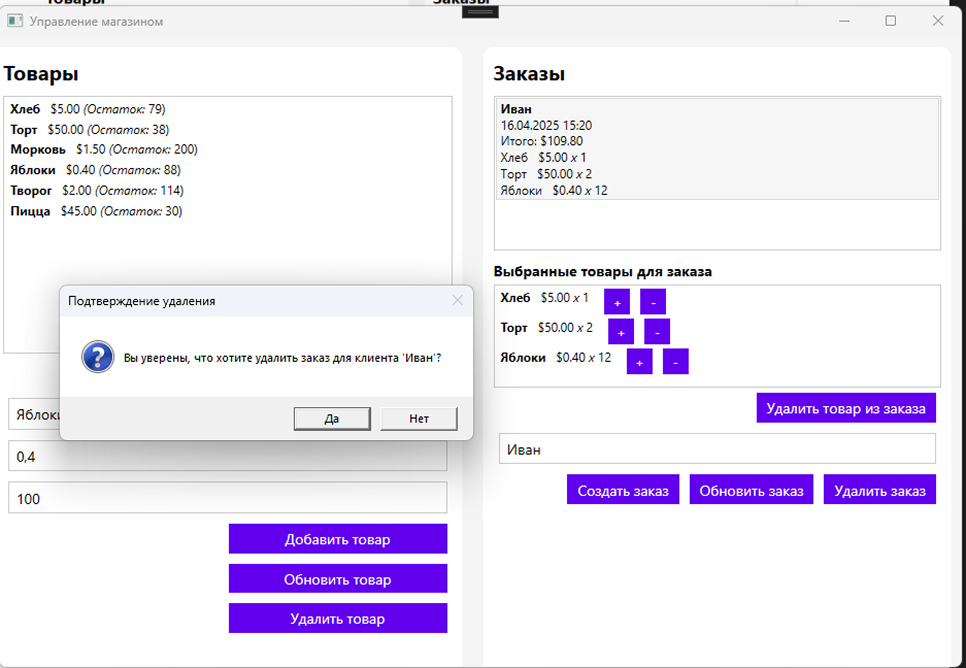
\includegraphics[width=1.0\textwidth]{fig/image 66.png}
	\caption{Удаление заказа} % Updated caption
	\label{fig:demo9}
\end{figure}

\pagebreak


При нажатии кнопки «Удалить товар из заказа» можно удалить конкретный товар, добавленный в заказ (Рисунок \ref{fig:demo10}).


\begin{figure}[ht]
	\centering
	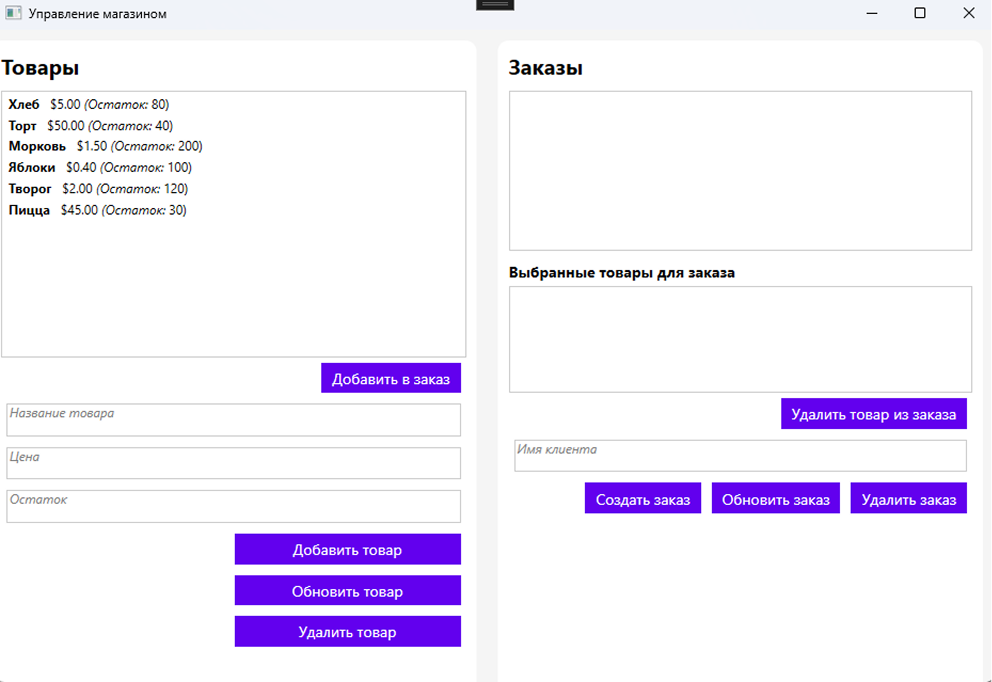
\includegraphics[width=1.0\textwidth]{fig/image 67.png}
	\caption{Удаление товара из списка выбранных товаров для заказа} % Updated caption
	\label{fig:demo10}
\end{figure}


\pagebreak

\section{ВОПРОСЫ ДЛЯ ЗАЩИТЫ~\texorpdfstring{\icon{}}{}}
\begin{enumerate}
	\item Вопрос
	\item Вопрос
	\item Вопрос
	\item Вопрос
	\item Вопрос
	\item Вопрос
	\item Вопрос
	\item Вопрос
	\item Вопрос
	\item Вопрос
\end{enumerate}

\end{document}
